g% --- Template for thesis / report with tktltiki2 class ---

\documentclass[finnish]{tktltiki2}

% tktltiki2 automatically loads babel, so you can simply
% give the language parameter (e.g. finnish, swedish, english, british) as
% a parameter for the class: \documentclass[finnish]{tktltiki2}.
% The information on title and abstract is generated automatically depending on
% the language, see below if you need to change any of these manually.
% 
% Class options:
% - grading                 -- Print labels for grading information on the front page.
% - disablelastpagecounter  -- Disables the automatic generation of page number information
%                              in the abstract. See also \numberofpagesinformation{} command below.
%
% The class also respects the following options of article class:
%   10pt, 11pt, 12pt, final, draft, oneside, twoside,
%   openright, openany, onecolumn, twocolumn, leqno, fleqn
%
% The default font size is 11pt. The paper size used is A4, other sizes are not supported.
%
% rubber: module pdftex

% --- General packages ---

\usepackage[utf8]{inputenc}
\usepackage{lmodern}
\usepackage{microtype}
\usepackage{amsfonts,amsmath,amssymb,amsthm,booktabs,color,enumitem,graphicx}
\usepackage[pdftex,hidelinks]{hyperref}

% Automatically set the PDF metadata fields
\makeatletter
\AtBeginDocument{\hypersetup{pdftitle = {\@title}, pdfauthor = {\@author}}}
\makeatother

% --- Language-related settings ---
%
% these should be modified according to your language

% babelbib for non-english bibliography using bibtex
\usepackage[fixlanguage]{babelbib}
\selectbiblanguage{finnish}

% add bibliography to the table of contents
\usepackage[nottoc,numbib]{tocbibind}
% tocbibind renames the bibliography, use the following to change it back
\settocbibname{Lähteet}

% --- Theorem environment definitions ---

\newtheorem{lau}{Lause}
\newtheorem{lem}[lau]{Lemma}
\newtheorem{kor}[lau]{Korollaari}

\theoremstyle{definition}
\newtheorem{maar}[lau]{Määritelmä}
\newtheorem{ong}{Ongelma}
\newtheorem{alg}[lau]{Algoritmi}
\newtheorem{esim}[lau]{Esimerkki}

\theoremstyle{remark}
\newtheorem*{huom}{Huomautus}


% --- tktltiki2 options ---
%
% The following commands define the information used to generate title and
% abstract pages. The following entries should be always specified:

\title{Ketterien menetelmien ratkaisuja ohjelmistotuotannon ja suunnitelmavetoisten menetelmien ongelmiin}
\author{Jarl-Erik Malmström}
\date{\today}
\level{Kandidaatintutkielma}
\abstract{Suunnitelmavetoiset menetelmät eivät sovi nopeasti muuttuvaan internet-aikakauden liiketoimintaympäristöön. Tarvitaan nopeasti reagoivia ja mukautuvia kehitysmenetelmiä. Ketterät menetelmät tarjoavat ratkaisuja muuttuviin vaatimuksiin ohjelmistokehityksen aikaisella kevyellä suunnitteluprosessilla. Ketterillä menetelmillä voidaan laatua unohtamatta toteuttaa käyttäjien toiveita vastaava ohjelmistojärjestelmä. Osa ketterien menetelmien käytänteistä parantaa ohjelmiston laatua.}

% The following can be used to specify keywords and classification of the paper:

\keywords{agile, ketterä, iteraatiivinen, ohjelmistotuotantomenetelmät, ongelmat, haasteet, ratkaisut. laatu}
\classification{} % classification according to ACM Computing Classification System (http://www.acm.org/about/class/)
                  % This is probably mostly relevant for computer scientists

% If the automatic page number counting is not working as desired in your case,
% uncomment the following to manually set the number of pages displayed in the abstract page:
%
% \numberofpagesinformation{16 sivua + 10 sivua liitteissä}
%
% If you are not a computer scientist, you will want to uncomment the following by hand and specify
% your department, faculty and subject by hand:
%
% \faculty{Matemaattis-luonnontieteellinen}
% \department{Tietojenkäsittelytieteen laitos}
% \subject{Tietojenkäsittelytiede}
%
% If you are not from the University of Helsinki, then you will most likely want to set these also:
%
% \university{Helsingin Yliopisto}
% \universitylong{HELSINGIN YLIOPISTO --- HELSINGFORS UNIVERSITET --- UNIVERSITY OF HELSINKI} % displayed on the top of the abstract page
% \city{Helsinki}
%


\begin{document}

% --- Front matter ---

\maketitle        % title page
\makeabstract     % abstract page

\tableofcontents  % table of contents
\newpage          % clear page after the table of contents


% --- Main matter ---

\section{Johdanto}
 
Ohjelmistotuotannossa (software development) käytetään työn suunnitteluun ja organisointiin ohjelmistotuotantomenetelmiä (software development methodologies). Menetelmät määrittelevät muodollisen prosessin, jonka lopputuloksena syntyy toimiva ohjelmistojärjestelmä.

Ohjelmistotuotannon alkuaikoina tietokoneet olivat kookkaita sekä niiden käyttö\-kustannukset olivat ohjelmistoja tuottavien insinöörien palkkoihin verrattuna korkeat. Korkeista kustannuksista johtuen ohjelmistotuotannossa tarvittiin suunnittelua sekä järjestelmällisiä käytäntöjä. Tietojenkäsittelyä ei tutkittu itsenäisenä tieteenalana, ja ohjelmistojen parissa työsken\-televät olivat muiden alojen insinöörejä sekä matemaatikkoja. Menetelmät olivat omaksuttu muista insinööritieteistä \cite{BOE06}.

Ohjelmistojen merkityksen kasvaessa ihmisten ja tietokoneiden vuorovaikutus korostui yhä enemmän. Ohjelmistoalalle tarvittiin lisää ihmisiä tuottavaan ja luovaan työhön sekä enemmän insinöörejä ja matemaatikkoja kuin oli saatavilla. Ohjelmistotuotantoprojekteihin palkattiin muiden alojen asiantuntijoita, jotka omaksuivat helposti \textit{ohjelmoi ja korjaa} (code and fix) lähestymistavan insinööri\-menetelmien sijasta \cite{BOE06}. Ohjelmoi ja korjaa mallissa ohjelmoidaan ensin ja mietitään vaatimuksia, rakennetta sekä testausta myöhemmin .\cite{BOE88}.

Ohjelmistotuotannon parissa työskentelevät huomasivat, että ohjelmiston kehitykseen liittyvät ilmiöt poikkesivat huomattavasti laitteistoihin liittyvistä ilmiöistä. Laitteistoille laadituilla luotettavuusmalleilla ei voitu arvioida ohjelmistojen luotettavuutta kattavasti. Ohjelmistoprojektien aikatauluja oli vaikea ennakoida, ja henkilöstön lisääminen aikataulun nopeuttamiseksi saattoi myöhästyttää projektia entisestään \cite{BOE06}.

Eroavaisuudet perinteisten insinöörimenetelmien ja ohjelmoi ja korjaa asenteiden välillä loi uutta hakkerikulttuuria merkittävien yliopistojen tietojenkäsittelylaitoksille. Nämä auktoriteetteja vastustavat luovat sankari ohjelmoijat tekivät usein vaikeasti muutettavaa ja ylläpidettävää ohjelmakoodia \cite{BOE06}. Tällainen menetelmä saattoi toimia jos tuotettava ohjelmisto on pieni, mutta järjestelmän kasvaessa uusien toiminnallisuuksien lisääminen vaikeutui. Lisäksi virheiden löytäminen ja korjaaminen vaikeutui järjestelmän kasvaessa \cite{FOW01a}.

Ohjelmistotuotantoon tarvittiin paremmin organisoituja menetelmiä ja kurinalaisia käytäntöjä yhä suurempien projektien hallinointiin. Reaktiona ohjelmoi ja korjaa menetelmille kehitettiin uusia prosessimalleja, joilla pyrittiin parantamaan 1950-luvun insinöörimenetelmien käytänteitä ohjelmistotuotantoon liittyvillä tekniikoilla. Prosessimalleissa ohjelmointia edelsi kattava suunnittelu- ja analysointivaihe\cite{BOE06}.

Internetin laajentuminen ja \textit{hypertekstijärjestelmän} (World Wide Web) ilmaantuminen korostivat ohjelmistojen merkitystä. Ohjelmistojen merkitys kilpailutekijänä ja liiketoimintaympäristön nopeutuminen lisäsivät tarvetta lyhentää ohjelmistotuotantoon kuluvaa aikaa. Suunnittelua, määrittelyä ja dokumentointia painottavat menetelmät eivät sopineet jatkuvasti muuttuvaan liiketoimintaympäristöön ja nopeaan ohjelmistokehitykseen (rapid application development)\cite{BOE06}.  

Ketterät menetelmät ovat olleet reaktio dokumentti- ja suunnitelmavetoisille menetelmille. Ketterät menetelmät pyrkivät kompromissiin, ohjelmoi ja korjaa-menetelmän ja raskaan menetelmän väliltä, tarjoamalla riittävän prosessin haluttuun lopputulokseen pääsemiseksi \cite{FOW01a}. Ketterissä menetelmissä korostetaan ihmisten välistä viestintää, sekä yhteistoimintaa niin ohjelmoijien kesken kuin asiakkaan kanssa. Ketterien menetelmien keskeisiä arvoja ovat luottamus ihmisten taitoihin sekä heidän sitoutumiseen omaan työhönsä \cite{COH01}.

Tässä tutkielmassa tarkastelemme ohjelmiston laatuun liittyviä käsitteitä ja ohjelmistotuotannon haasteita seuraavassa kappaleessa. Käymme läpi erilaisia suunnitelmavetoisia ja ketteriä menetelmiä sekä näiden lähestymistapoja ohjelmistotuotantoon kappaleessa kolme. Kappaleessa neljä tutkimme suunnitelmavetoisten prosessimallien hyötyjä ohjelmistotuotannon haasteisiin ja selvitämme miten ketterät menetelmät ovat pyrkineet ratkaisemaan suunnitelmavetoisten prosessimallien heikkouksia, ohjelmistotuotannon haasteita ja ohjelmiston laatuun liittyviä ongelmia. 

\section{Ohjelmistotuotannon haasteet ja laatu}

Ohjelmistotuotantoprojekteissa saattaa ilmetä monia haasteita projektin koordinointiin tai ohjelmistolta odotettuun toiminnallisuuteen liittyen. Ohjelmistotuotannossa ilmenevät haasteet voidaan jakaa seuraaviin osa-alueisiin: henkilöstön hallinta, projektin aikataulu ja taloudelliset resurssit, vaatimusten hallinta, tekniset valmiudet ja projektin mahdolliseen ulkoistukseen liittyvät ongelmat \cite{BOE88}.

Ongelmia  ohjelmistoprojekteissa ilmenee, kun ohjelmistoprojektiin on palkattu liian vähän pätevää henkilöstöä tai ohjelmiston kehityksen aikataulu tai budjetti ovat arvioitu väärin \cite{BOE88}. 

Ohjelmiston toimintaympäristön ja operatiivisen käytön kattava analysointi ja määrittely ennen ohjelmointia on vaikeaa. Tästä johtuen, ohjelmistoon usein kehitetään toiminnallisuuksia, joita ei tarvita tai ne ovat väärin määriteltyjä. Ohjelmoijat voivat myös ammatillisesta kiinnostuksesta lisätä tarpeettomia toiminnallisuuksia. Vähäisestä asiakasyhteistyöstä johtuen järjestelmään saatetaan kehittää puutteellinen tai vaikea käyttöliittymä \cite{BOE88}. 

Ongelmia saattaa aiheuttaa rakennetun järjestelmän odotettua heikompi suorituskyky. Toisaalta tietotekniset mahdollisuudet voidaan arvioida väärin eikä käytössä olevien tietokoneiden laskentakyky riitä suunniteltuun järjestelmään \cite{BOE88}.


\subsection{Koordinointi}

Tässä tutkielmassa koordinoinnilla tarkoitamme yksilöiden ja ryhmien välistä yhteistoimintaa sekä näihin liittyvää hallinnollista työtä ja toisaalta ohjelmistojärjestelmän eri osien yhteensovittamista sekä ohjelmistoprojektin hallinnointia. Ohjelmistoprojektin koordinointiongelmat liittyvät henkilöstön ja vaatimusten hallintaan sekä ulkoistettuun ohjelmistotuotantoon \cite{KES95}. 

Yksilöiden tai ryhmän on mahdotonta luoda tai ymmärtää suuria ohjelmistoja yksityiskohtaisesti. Suuriin ohjelmistoprojekteihin saattaa liittyä useita kehittäjä\-organisaatioita ohjelmiston tilaajan lisäksi. Suuret projektit onnistuvat useimmin jos projektia koordinoi henkilö, jolla on tietoa ohjelmiston kohdealueelta sekä ohjelmistoalalta. Ohjelmiston kohdealueen tietoa katoaa suurissa ohjelmistotuotantoprojekteissa, joissa ohjelmistokoodin koko voi olla miljoonia rivejä ja ohjelmistoprojektin kesto useita vuosia. Suuret projektit johtavat erikoistumiseen ja työn jakamiseen. Organisaatiossa tämä johtaa toisistaan riippuvien tekijöiden jakamiseen osastoihin maantieteellisesti, organisatorisesti, sekä sosiaalisesti. Tämä vähentää mahdollisuuksia ja haluja oppia sekä jakaa tietoa etäisten työtovereiden kesken\cite{KES95}.

Suuri kokoluokka ja epävarmuus aiheuttavat ongelmia, koska ohjelmisto vaatii sen osajärjestelmien täsmällistä integraatiota. Ohjelmistot ovat pääasiallisesti rakennettu useista osista, jotka on kytkettävä yhteen, jotta ohjelmisto toimisi oikein \cite{KES95}. Ohjelmistojen monimutkaisuus tekee määrittelystä ja testaamisesta vaikeaa\cite{BOE06}. 

Toisaalta koordinointiongelma liittyy ohjelmistoa kehittävän organisaation ja asiakkaan väliseen yhteistyöhön: asiakkaalla on vaatimuksia kehitettävän järjestelmän toiminnallisuuksista, joita ohjelmoijat toteuttavat. Vaikeuksia ilmenee näiden vaatimuksien ymmärtämisessä ja usein vaatimukset muuttuvat projektin edetessä \cite{FOW01a}. 

\subsection{Suunnittelu ja muuttuvat vaatimukset}

Ohjelmistotuotannon koordinointi vaikeutuu ja epävarmuus lisääntyy, koska ohjelmiston toimintaan liittyvät vaatimukset muuttuvat ohjelmistoprojektin edetessä. Muutoksia ohjelmiston vaatimuksiin esiintyy, koska liiketoiminta, käyttäjien toiveet, tietokoneympäristö, ohjelmiston syötteet ja fyysinen maailma muuttuvat \cite{KES95}.

Muutostarpeiden ilmaantumisen todennäköisyys on suurin, kun käyttäjät käyttävät toimivaa ohjelmistoa. Tällöin käyttäjät näkevät ohjelmiston rajoitteet ja mahdollisuudet. Kun ihmiset käyttävät ohjelmistoa, niin he todennäköisesti vaativat uusia toiminnallisuuksia \cite{KES95}. Ohjelmiston toiminnallisuuksien arvoja on vaikea nähdä ennen kuin ohjelmistoa käytetään oikeassa toimintaympäristössä \cite{FOW01a}.

Tyypillisesti ohjelmistotuotantoprojektiin osallistuva henkilö vaihtelevalla kohdealueen tuntemuksella haastattelee asiakkaita ja käyttäjiä. Tämän jälkeen hän kirjoittaa vaatimukset ohjelmistoarkkitehdeille ja -suunnittelijoille, jolloin merkityksellistä kohdealueen tietoa katoaa \cite{KES95}.

Vaatimusmäärittelyssä kaikkia käyttäjien tarpeita ei löydetä ja jotkin tarpeet jäävät kirjaamatta. Suuri haaste ohjelmistokehityksessä on, että ohjelmistoarkkitehtien ja -suunnittelijoiden päätöksentekoon tarvitsema tieto ei ole saatavilla \cite{KES95}.  

Muuttuvat tai puutteelliset vaatimukset voidaan nähdä johtuvan heikosta suunnittelusta ja vaatimusmäärittelystä. Suunnitelmavetoisissa menetelmissä vaatimusmäärittelyn tarkoituksena on selkeä kokonaiskuva toteutettavista toiminnallisuuksista ennen ohjelmiston rakentamista, saada asiakas allekirjoittamaan sopimus toteutettavista toiminnallisuuksista ja rajoittaa asiakkaan vaatimia muutoksia sopimuksen allekirjoituksen jälkeen \cite{FOW01a}.

Vaatimusten ja toiminnallisuuksien hallinnoinnin ongelmana on, että erilaisten vaihtoehtojen vertailu on vaikeaa, koska ohjelmistokehittäjät eivät yleensä tarjoa hinta-arvioita erilaisista toiminnallisuuksista. Ilman tietoa hinnasta on vaikea arvioida halutaanko tietystä toiminnallisuudesta maksaa. Arviointi on vaikeaa, koska ohjelmistokehitys on suunnittelutyötä. \cite{FOW01a}. Toisin kuin teollinen valmistus, ohjelmistokehitys ei ole rutiininomainen toimi: ohjelmistoprojektit ovat yksilöllisiä eikä ohjelmistojärjestelmille yleensä ole valmiita protyyppejä \cite{KES95}.

Teknologian ja liiketoiminnan vaatimusten muuttuessa vaatimusmäärittelyt ja suunnitelmat vanhentuvat nopeasti \cite{WIC03}. Alkuperäisen vaatimusmäärittelyn ja suunnitelman seuraaminen ei ole ohjelmistoprojektien päämäärä, sen sijaan toimitettavan ohjelmiston tarkoitus on asiakkaan mahdollisesti muuttuvien tarpeiden tyydyttäminen \cite{HIC01}. Internet liiketoimintaympäristönä vahvistaa ohjelmistotuotannon ongelmia korostamalla nopeutta. Asiakkailla on epätoivoinen kiire markkinoille. He vaativat liiketoiminnalle arvoa tuottavia ominaisuuksia yhä nopeammassa tahdissa. \cite{BRL03}.

Ohjelmistokehitys on epävarmaa, koska vaatimukset ovat epätäydellisiä. Epätäydellisyys johtuu osittain ohjelmistoprojektin työn jakautumisesta eri organisaatioihin.
Suurissa ohjelmistoprojekteissa on monia organisaatioita ja kehittäjätiimejä. Vaatimusmäärittelyn, suunnittelun ja toteutuksen tekevät eri ihmiset. Joillakin projektiin osallistuvilla ei ole riittävää tuntemusta kohdealueesta ja liiketoimintaympäristöstä \cite{KES95}.


\subsection{Tekninen kehitys ratkaisuna}

Käytännön kokemus osoittaa, että aikaisempi ohjelmistotuotannon kehitys ei ole onnistunut ratkaisemaan suurien ohjelmistoprojektien haasteita. 
Voidaan sanoa, että aikaisemmat korjaustoimenpiteet ovat lähestyneet ongelmia seuraavasti: 
\begin{itemize}
 \item Kehittämällä ohjelmistotuotannossa tarvittavia teknisiä työkaluja.
 \item Jakamalla ohjelmisto osiin (modularization) teknisesti, esimerkiksi olio-ohjelmoinnilla (object-oriented programming). 
 \item Jakamalla ohjelmistotuotantoa hallinnollisesti: eriyttämällä vaatimusmäärittelyn, ohjelmoinnin ja testaustoiminnot.
 \item Formalisoimalla teknisiä menettelytapoja, esimerkiksi versionhallinta, testisuunnitelma ja vaatimusmäärittelydokumentit \cite{KES95}.
\end{itemize}

Nykyään ohjelmistokehittäjät käyttävät laajasti työkaluja, jotka nopeuttavat suunnittelu- ja ohjelmointiprosessia. Uuden teknologian työkalut tarjoavat toimintoja, jotka ennen oli toimitettava itse. Erilaiset ohjelmistokehykset (frameworks) tekevät osan ohjelmiston kehitystä. Ohjelmistokehitystä voidaan nopeuttaa komponenttien uudelleenkäytöllä. Sen sijaan, että rakennettaisiin ohjelmisto alusta alkaen itse, valmiita komponentteja hankintaan, yhdistetään ja kootaan nopeasti \cite{BRL03}.

Nykyiset ohjelmistotyökalut eivät ole tarjonneet yksiselitteisiä ratkaisuja ohjelmistotuotannon haasteisiin: miten tuottaa toimiva vaatimusten mukainen ohjelmistojärjestelmä ajallisia ja taloudellisia resursseja ylittämättä. Työkalut lisäävät yksilöiden tuottavuutta, mutta eivät ratkaise ohjelmistotuotannon koordinointiongelmaa. Yhdessä työskentelevien ihmisten ja heidän erilaiset näkemykset on sovitettava yhteen onnistuneen ohjelmiston luomiseksi \cite{KES95}.

Seuraavaksi tarkastelemme tässä kappaleessa ohjelmiston laatuun liittyviä määritelmiä ja miten ohjelmistotuotannon haasteet heijastuvat ohjelmiston laatuun. Kappaleessa kolme selvitämme miten suunnitelmavetoiset menetelmät ovat pyrkineet ratkaisemaan ongelmia.

Ohjelmistokehittäjien on otettava laatu huomioon sekä suurissa monimutkaisissa ohjelmistojärjestelmissä että pienissä sulautetuissa ohjelmistoissa. Ohjelmistossa ilmeneviä virheitä sallitaan enemmän tekstinkäsittelyohjelmassa kuin ydinvoimalalaitoksen ohjausjärjestelmissä \cite{KIP96}.

Oletetaan, että tilattu ohjelmistojärjestelmä toimitetaan ajallaan ilman budjettia ylittäviä kustannuksia, ja se toimii oikein sekä suorittaa tehokkaasti sille määritetyt toiminnallisuudet. Voidaanko tuotteeseen tällöin olla tyytyväisiä? Ei välttämättä kaikissa tapauksissa. Ohjelmistojärjestelmää voi olla vaikea ymmärtää ja muuttaa. Ohjelmistoa ei välttämättä ole helppokäyttöinen. Ohjelmisto voi olla tarpeettoman laitteistoriippuvainen. Nämä seikat johtavat kohtuuttomiin ylläpitokustannuksiin \cite{BBL76}.

Ohjelmiston laatu on vaikea käsite, koska laatu tarkoittaa eri asioita eri ihmisille. Eikä laadun mittaamiseen ole yhtä kaikkien hyväksymää mittaria \cite{KIP96}.        

Kansainvälinen standardointi organisaatio (ISO) on suositellut laadun perustaksi kuusi itsenäistä piirrettä:

\begin{enumerate}
  \item toiminnallisuus (functionality)
  \item luotettavuus (reliability)
  \item käytettävyys (usability)
  \item tehokkuus (efficiency)
  \item ylläpidettävyys (maintainability)
  \item siirrettävyys (portabilty) \cite{KIP96}
\end{enumerate}

Tuotettavan ohjelmiston toiminnallisuus ja luotettavuus määritellään seuraavasti: toiminnallisuuksien on tyydytettävä käyttäjän vaatimukset sekä kyettävä ylläpitämään vaadittu suorituskyky vaaditun ajan. Käytettävyyden on vastattava oletettua ohjelmiston käytöstä aiheutuvaa vaivannäköä. Tehokkuudella tarkoitetaan suorituskyvyn ja käytettyjen resurssien suhdetta. Yllä\-pidettävyys määritellään ohjelmistoon tehtäviin muutoksiin tarvittavalla työmäärällä, jotka voivat liittyä korjauksiin, parannuksiin tai ohjelmiston mukauttamista muuttuneisiin olosuhteisiin. Siirrettävyys viittaa ohjelmiston kykyyn toimia erilaisessa ympäristössä: toisessa organisaatiossa, laitteistossa tai ohjelmistoympäristössä \cite{KIP96}.

Yllä mainitut ISO:n laatumallin piirteistä liittyvät käyttäjän näkemykseen (user view) ohjelmistosta ja miten se tyydyttää hänen tarpeensa. Toisaalta tuotettavan ohjelmistojärjestelmän vaatimuksia edustaa käyttäjän tai asiakkaan tarpeet ja näkemys, joten aikaisemmin tässä kappaleessa esiin tuomamme ohjelmistotuotannon haasteet kytkeytyvät oleellisesti ohjelmiston laatuun. Vaatimusten hallinta voidaan näin nähdä liittyvän ohjelmiston laadun hallintaan \cite{KIP96}. 

Seuraavaksi tarkastelemme suunnitelmavetoisia menetelmiä sekä ketteriä menetelmiä ja niiden lähestymis\-tapoja ohjelmistotuotannon haasteisiin ja toisaalta laatuun, koska edellä totesimme niiden liittyvän toisiinsa. Käymme ensin lyhyesti läpi lineaarisen ja iteratiivisen ohjelmistotuotantomenetelmän sekä näiden menetelmien ongelmia.

\section{Suunnitelmavetoiset menetelmät ja ketterät menetelmät}

Suunnitelmavetoiset ohjelmistotuotantomenetelmät ovat ohjelmistokehityksen yksityiskohtaisia ja kurinalaisia prosesseja, joiden tarkoituksena on tehdä ohjelmistotuotannosta ennustettavaa ja tehokasta sekä välttää ohjelmistotuotantoon liittyviä riskejä. Muista insinööritieteistä vaikutteita saaneet menetelmät ovat yksityiskohtaisia prosesseja, joissa painotetaan suunnittelua\cite{FOW01a}.

\subsection{Vesiputousmalli}

Vesiputousmalli (waterfall model) on lineaarinen vaiheesta seuraavaan etenevä prosessimalli. Vesiputousmallissa ohjelmistotuotanto koostuu seuraavista vaiheista: järjestelmän ja ohjelmiston vaatimusmäärittely sekä analyysi, ohjelmistonrakenteen suunnittelu, ohjelmointi, testaus ja ohjelmiston käyttö \cite{ROY70}.

1970-luvulla vesiputousmalli vaikutti suuresti lineaarisiin ohjelmistotuotannon suunnitelmavetoisiin prosessimalleihin. Vesiputousmallin lähestymistapa auttoi poistamaan monia aiemmin ohjelmistotuotantoa vaivanneita ongelmia \cite{BOE88}.

\begin{figure}[h!]
  \caption{Lineaarinen ohjelmistotuotantoprosessi}
  \centering
    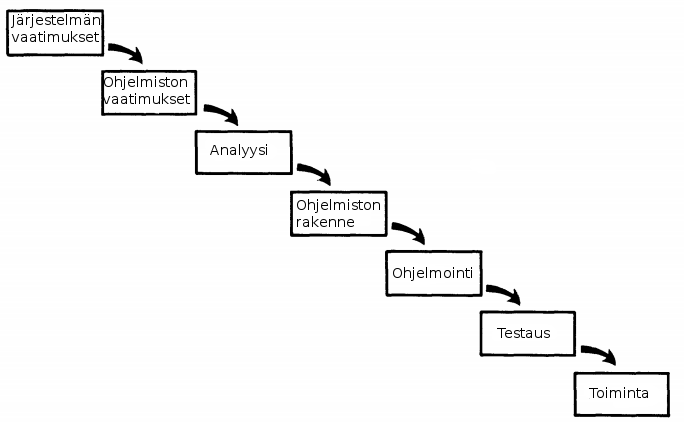
\includegraphics[width=\textwidth]{waterfall}
\end{figure}

Kuvassa 1. on kuvaus lineaarisesta vesiputousmallista.

Määrittely- ja analyysivaiheessa kerätään kehitettävän järjestelmän ja ohjelmiston vaatimukset ja rajoitteet. Vaatimukset ovat joukko toiminnallisuuksia, joita loppukäyttäjä odottaa ohjelmistolta. Loppukäyttäjien vaatimuksien ja liiketoimintaympäristön analysointi on edellytys ohjelmiston rakenteen suunnittelulle. \cite{ROY70}.

Seuraavassa vaiheessa suunnitellaan järjestelmän rakenne: ohjelmiston arkkitehtuuri, tarvittavat luokat ja niiden toiminnallisuus sekä komponenttien yhteensopivuus ja yhteistoiminta. \cite{ROY70}.

Ohjelmointivaiheessa kirjoitetaan ohjelmakoodi laadittujen suunnitelmien perusteella. Testausvaiheessa varmistetaan, että rakennettu ohjelmistojärjestelmä toimii vaatimusten mukaan. Toimintavaiheessa ohjelmisto on loppukäyttäjillä operatiivisessa toiminnassa \cite{ROY70}. 

Testauksen tulisi tehdä siihen erikoistuneet henkilöt, jotka eivät välttämättä ohjelmoineet itse alkuperäistä ohjelmiston osaa. Useimmat virheet ovat luonteeltaan ilmiselviä, jotka voidaan löytää visuaalisella tarkastelulla. Jokaisen analyysin ja ohjelmakoodin tulee tarkastaa toinen henkilö, joka ei osallistunut varsinaiseen työhön. Jokainen tietokoneohjelman looginen polku on testattava ainakin kerran \cite{ROY70}.

Vesiputousmallissa painotetaan dokumentin tärkeyttä, jotta testaaja voisi ymmärtää ohjelmiston toimintaa. Hyvän dokumentoinnin todellinen arvo ilmenee testausvaiheessa, ohjelmistoa käytettäessä sekä uudelleen suunniteltaessa. Hyvän dokumentin avulla esimies voi keskittää henkilöstön ohjelmistossa ilmenneisiin virheisiin. Ilman hyvää dokumenttia, ainoastaan ohjelmistovirheen alkuperäinen tekijä kykenee analysoimaan kyseessä olevan virheen. Käyttöönotossa ilmenneiden ohjelmistovirheiden korjaamisessa selkeä dokumentti on välttämätön \cite{ROY70}.

Vesiputousmallin ongelmana oli dokumentaation korostuminen valmistumiskriteerinä aikaisille vaatimuksille ja suunnitteluvaiheille. Menetelmä ei sovi interaktiivisiin loppukäyttäjien sovelluksiin, koska käyttäjät näkevät lopputuloksen ohjelmistotuotantoprojektin loppuvaiheessa. Dokumenttivetoisuus pakottaa kirjaamaan yksityiskohtaisesti heikosti ymmärretyt käyttö\-liittymien vaatimukset. käyttäjät eivät kykene tyhjentävästi kertomaan mitä toiminnallisuuksia ohjelmistolta haluavat. Asiakas saattaa muuttaa mielensä. Tai hän osaa usein sanoa, nähdessään valmiin tuotteen, mitä olisi ohjelmistolta halunnut \cite{BEC99}.

Muuttuvista vaatimuksista seuraa käyttökelvottoman ohjelmakoodin suunnittelua ja toteutusta. Lineaarisen ohjelmistotuotantomenetelmän vaiheet ovat tällaisille projekteille selvästi väärässä järjestyksessä. Joillekin ohjelmistoille ei ole tarvetta yksityiskohtaiselle dokumentaatiolle ennen toteutusta \cite{BOE88}.

Ongelmana ohjelmistotuotannossa on, että muutosten kustannukset kasvavat ohjelmiston elinkaaren aikana. Mitä pidemmälle projekti etenee sitä kalliimpaa muutosten tekeminen on \cite{HIC01}.


\subsection{Spiraalimalli}

Spiraalimallin (spiral model) tarkoitus oli edistää ohjelmistotuotantoprosessia lähestymällä ohjelmistoa iteratiivisesti (iterative) ja inkrementaalisesti (incremental) sekä analysoimalla tuotannossa kohdattavia haasteita. Tämä mahdollistaa mallin mukautumaan, kohdattavien riskien mukaan, sopivasti yhdistelemällä määrittelyä (specification), prototyyppien valmistusta, simulointia tai muita lähestymistapoja ohjelmiston suunnitteluun. Spiraalimalli on kehitetty vesiputousmallista saatujen useiden vuosien kokemuksien perusteella, ja se ratkaisi vesiputousmallin monia puutteita \cite{BOE88}.


Kuvassa 2. oleva spriraalimalli kuvastaa taustalla olevaa käsitettä, että jokainen vaihe sisältää saman sarjan toimenpiteitä \cite{BOE88}.

\begin{figure}[h!]
  \caption{Spiraalimallin ohjelmiston elinkaari}
  \centering
    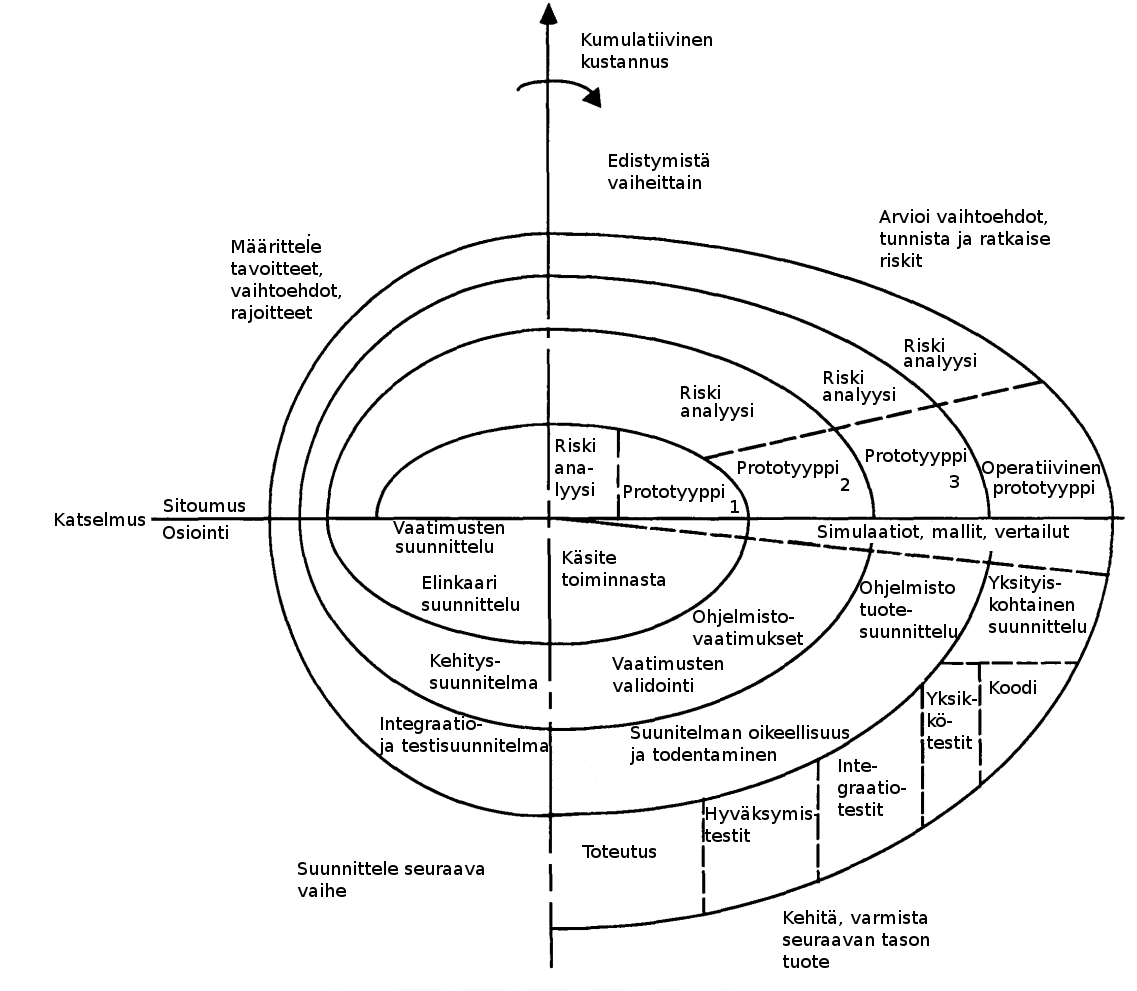
\includegraphics[width=\textwidth]{spiral}
\end{figure}

Spiraalimallissa jokainen vaihe aloitetaan tunnistamalla:
\begin{itemize}
  \item laadittavien ohjelmisto-osien suorituskykyyn, toiminnallisuuteen sekä sopeutumiskykyyn liittyvät tavoitteet
  \item vaihtoehtoiset toteutustavat (ohjelmiston osto, ohjelmiston uudelleenkäyttö, vaihtoehtoiset ohjelmat)
  \item ohjelmiston eri vaihtoehdoille asettamien rajoitteet (rajapinnat, aikataulu, kustannukset) \cite{BOE88}.
\end{itemize}

Seuraava askel on arvioida vaihtoehtoja suhteessa ohjelmiston tavoitteisiin ja rajoitteisiin. Usein tämä prosessi tunnistaa epävarmoja alueita, jotka ovat merkittäviä riskin lähteitä. Riskien löytyessä, seuraava askel pitää sisällään kustannustehokkaan strategian muotoilun riskien ratkaisemiseksi. Tähän voi liittyä prototyyppien valmistamista, simulointia, vertailuanalyysia, kyselylomakkeita, analyyttista mallinnusta, tai näiden yhdistelmiä sekä muita riskien ratkaisumenetelmiä \cite{BOE88}.

Jos suorituskykyyn tai käyttöliittymään liittyvät riskit hallitsevat ohjelman kehittämistä, seuraavassa vaiheessa määritellään ohjelmiston yleistä luonnetta, suunnitellaan seuraavan tason prototyyppiä ja kehitetään yksityiskohtaisempaa prototyyppiä riskien ratkaisemiseksi \cite{BOE88}.

Riskinhallinta huomioiden voidaan määritellä kiinnitettävä aika ja työmäärä toiminnan suunnitteluun (planning), asetuksien hallintaan (configuration management), laadun varmistukseen (quality assurance), muodolliseen todentamiseen (formal verification) ja testaukseen \cite{BOE88}.

Spiraalimallin tärkeä ominaisuus on, että jokainen iteraatio päätetään katselmukseen tuotteeseen liittyvän henkilöstön tai organisaation kanssa \cite{BOE88}.


Spiraalimallissa ei määritellä iteraatioiden pituutta suhteessa ohjelmistokehitykseen vaadittuun aikaan. Mallissa painotetaan vahvasti prototyypin osuutta ohjelmiston kehityskaaren aikana. Varhainen prototyyppi tarjoaa ohjelmiston testattavaksi, jotta virheitä voidaan löytää aikaisessa vaiheessa \cite{BOE88}.

Spriraalimallin riskien analysoinnista huolimatta, ohjelmiston kehitysprosessi sisältää haasteita ohjelmiston vaatimusten hallintaan, laatuun ja erityisesti testaukseen liittyen. Spriraalimallissa ohjelmiston testausta tehdään prototyypin kehityskaaren lopussa ja palautetta asiakkaalta saadaan vasta iteraation lopussa. Spriraalimallissa ei ole korostettu vaatimuksien tärkeys\-järjestystä ja hallinointia ei ole korostettu \cite{BOE88}. Aikaisemmin totesimme vaatimusten ja laadun hallinnan liittyvän toisiinsa \cite{KIP96}. 

Seuraavaksi tarkastelemme ketteriä kehitysmenetelmiä sekä miten nämä menetelmät ovat pyrkineet ratkaisemaan aikaisemmin käsiteltyjen menetelmien puutteita ja miten ketterät menetelmät lähestyvät ohjelmistotuotannon haasteita ja ohjelmiston laatua. 

Ketterät menetelmät toivottavat muutokset tervetulleiksi, ja ohjelmisto kehittyy uusiin vaatimuksiin ja muutoksiin mukautuen \cite{WIC03}. Perinteinen lähestymistapa perustui oletukselle, että aikaisella ja täydellisellä vaatimusmäärittelyllä voidaan pienentää kustannuksia vähentämällä muutoksia. Nykyään muutosten kieltäminen merkitsee reagoimattomuutta liiketoimintaympäristön kehitykselle \cite{HIC01}.

Suunnitelmavetoisten prosessimallien ongelmien seurauksena useat ohjelmistoalan ihmiset ja organisaatiot kehittivät menetelmiä ja käytäntöjä, joille muutokset ovat hyväksyttyjä. 

Menetelmiä kehitettiin useita ja eri maissa: 
\begin{itemize}
 \item taipuisa järjestelmän kehitysmenetelmä (Dynamic Systems Development) Euroopassa
 \item toiminnallisuusvetoinen kehitysmenetelmä (Feature-Driven Development) Australiassa
 \item ja XP (Extreme Programming) \cite{BEC99}, Crystal \cite{COC05}, mukautuva ohjelmistokehitys (Adaptive Software Development) ja Scrum \cite{SCH09} Yhdysvalloissa \cite{WIC03}.
\end{itemize}

Eri menetelmien eroavaisuuksista huolimatta, kaikilla lähestymistavoilla oli yhteistä välttää, lineaarista vaihe kerrallaan etenevää, suunnitelma- ja dokumenttivetoista menetelmää \cite{LAB03}.

Helmikuussa 2001 17 menetelmien kehittäjää tapasi keskustellakseen kevyistä menetelmistä ja kokemuksiensa yhtäläisyyksistä. Huomatessaan, että heidän käytänteillään oli paljon yhteistä, ja että heidän prosessinsa tarjosivat keinoja saavuttaa merkityksellinen päämäärä: asiakkaan tyytyväisyys ja korkea laatu \cite{WIC03}. 

Osallistujat määrittelivät käytännöt ketteriksi menetelmiksi.
Osallistujat kirjoittivat ''Manifesto for Agile Software Development''-julistuksen, mikä kuvaa ketterän kehityksen perusarvoja:

\begin{itemize}
 \item yksilöt ja vuorovaikutus ennen prosesseja ja työkaluja
 \item toimiva ohjelmisto ennen kattavaa dokumentaatiota
 \item asiakasyhteistyö ennen sopimusneuvotteluja
 \item muutoksiin vastaaminen ennen suunnitelman seuraamista \cite{WIC03}.
\end{itemize}

Ohjelmistotuotannon parissa työskentelevät huomasivat, että ohjelmistoinsinööritieteet erosivat huomattavasti muista insinööritieteistä. Autojen kokoaminen on määriteltävä prosessi. Insinöörit voivat suunnitella prosessin, määritellä kokoonpanojärjestyksen sekä työntekijöiden, koneiden tai robottien toimenpiteet \cite{WIC03}.

Ohjelmistotuotantoprojektit ovat luonteeltaan empiirisiä prosesseja, joiden lopputuloksena syntyy uusia tuotteita. Projektin aikana on oleellista oppia ja mukautua prosessin edetessä, eikä määritellä kaikkea alussa kattavasti. Empiirinen prosessi vaatii \textit{tarkkaile ja mukaudu} (\textit{inspect and adapt}) tyyppisen lähestymistavan. Lyhyet iteraatiot auttavat ketteriä menetelmiä mukautumaan ja muuttamaan ohjelmistoteollisuuden ennustamattomien vaatimuksien mukaan \cite{WIC03}.

Kerromme seuraavaksi lyhyesti kahdesta ketterästä kehitysmenetelmästä. Selvitämme miten suunnittelua on lähestytty näissä menetelmissä ja miten niiden käytänteet ovat pyrkineet ratkaisemaan ohjelmistotuotannon haasteita ja laatuun liittyviä ongelmia. Käsittelemme näiden ketterien menetelmien ratkaisuja toisessa kappaleessa esitettyihin ohjelmistotuotannon haasteisiin. Tutkimme myös onko ketterillä menetelmillä ohjelmiston laatuun merkittävää vaikutusta.

\subsection{Extreme programming}

XP (Extreme Programming) vähentää ohjelmiston vaatimusten muuttumisen kustannuksia tekemällä koko kehityskaaren aikaisia toimintoja jatkuvasti ohjelmistokehityksen aikana. Perinteisen ohjelmistotuotantoprosessin sijaan suunnitellaan, analysoidaan ja muotoillaan rakennetta jokaisessa iteraatiossa \cite{BEC99}.

XP:ssä asiakas valitsee eniten arvoa tuottavat tarinat (story), jotka ovat arviotavissa ja testattavissa. Ohjelmoijat jakavat tarinat pieniksi tehtäviksi (task). Ohjelmoijat muuttavat tehtävät joukoksi testejä, jotka osoittavat tehtävän valmistuneen \cite{BEC99}. 

XP:n käytäntöihin kuuluu jatkuva pariohjelmointi (pair programming). Parin kanssa työskentelemällä ohjelmoijat ajavat testejä ja kehittävät samalla mahdollisimman yksinkertaista suunnitelmaa tehtävän ratkaisemiseksi \cite{BEC99}.  

\subsection{Scrum}

Scrum lähestyy ohjelmistotuotantoprojektin monimutkaisuutta joukolla yksinkertaisia käytänteitä ja sääntöjä. Scrum on tarkasteleva, mukautuva ja empiirinen prosessi. Scrum perustaa kaiken käytännön iteratiiviselle ja inkrementaaliselle prosessille. Jokaisen iteraation tulos on ohjelmistotuotteen inkrementaalinen edistyminen. Iteraatioita vie eteenpäin lista vaatimuksista \cite{SCH09}.

Iteraatioita kutsutaan sprinteiksi (sprint). Sprintti on 30 päivän iteraatio, jonka aika tuotetaan \textit{valmiin} (\textit{done}) määritelmän mukainen ohjelmisto. Sprintti aloitetaan sprintin suunnittelupalaverilla (sprint planning meeting), jossa valitaan kehitettävät toiminnallisuudet. Sprintin lopussa pidetään sprinttikatselmus (sprint review meeting), jossa ohjelmistoversio esitellään sidosryhmille \cite{SCH09}.

Scrumissa on projektissa kolme roolia: tuoteomistaja (Product owner), kehittäjätiimi (team) ja scrummaster (Scrum master). Tuoteomistaja on asiakasedustaja, joka rahoittaa ja visioi ohjelmistotuotteen. Kehittäjätiimi vastaa ohjelmiston toteuttamisesta ja scrummaster vastaa käytänteiden toteutumisesta ja opastaa kehittäjätiimiä saavuttamaan tavoitteensa \cite{SCH09}.

Scrum määrittelee neljä ohjelmistokehityksessä käytettävää tuotosta (artifact): tuotteen kehitysjono (product backlog), sprintin tehtävälista (sprint backlog), edistymiskäyrä (burndown chart) ja tuoteversio (increment of potentially shippable product functionality) \cite{SCH09}. 

Ohjelmistojärjestelmän vaatimukset listataan tuotteen kehitysjonossa, jota käytetään suunnittelussa ja vaatimusten hallinnassa koko ohjelmistokehitysprosessin ajan. Tuoteomistaja on vastuussa tuotteen kehitysjonon sisällöstä ja vaatimusten tärkeysjärjestyksestä \cite{SCH09}.

Sprintin tehtävälista sisältää tehtävät, jotka kehittäjätiimi inkrementoi julkaistavaksi tuotteen toiminnallisuudeksi. Sprintin tehtävälista on läpinäkyvä reaaliaikainen kuvaus työstä, jonka kehittäjätiimi suunnittelee saavansa valmiiksi sprintin aikana \cite{SCH09}.

Edistymiskäyrä ilmaisee visuaalisesti jäljellä olevan työmäärän ja ajan suhdetta. Edistymiskäyrällä voidaan peilata todellista työn edistymistä ja nopeutta projektin suunnitelmiin ja toiveisiin \cite{SCH09}.

Scrum vaatii kehitystiimiä rakentamaan uuden tuoteversion jokaisessa sprintissä. Tuoteversio on toimiva ohjelmisto, johon jokaisessa iteraatiossa on lisätty uusia täysin testattuja toiminnallisuuksia \cite{SCH09}.

\section{Ketterien menetelmien ratkaisuja}

\subsection{Suunnittelu, muuttuvat vaatimukset ja laatu}

Toisessa kappaleessa totesimme vaatimusten hallinnan olevan osa ohjelmistotuotannon koordinointiongelmaa. Kolmannessa kappaleessa käsittelimme ohjelmiston laatua ja yhdistimme laadun käsitteitä käyttäjän vaatimuksiin. 

Perinteinen suunnittelu on sisältänyt UML-kaavioita (unified modeling language), joilla voidaan kuvailla ohjelmiston rakennetta ja käyttäytymistä. Ketterien menetelmien prosesseissa suunnittelussa painotetaan joustavuutta, jotta suunnitelmaa voidaan helposti muuttaa kun vaatimukset muuttuvat \cite{FOW01b}.

XP:ssä suunnitelmien ja kaavioiden merkitys on vähäinen: UML kaavioita tulee käyttää, jos niistä on hyötyä. Äärimäiset XP:n toteuttajat eivät käytä UML-kaavioita lainkaan \cite{FOW01b}.

Kaavioiden merkitys on tarjota yhteydenpitoa. Tehokkaan yhteydenpidon takaamiseksi on piirrettävään kaavioon valittava tärkeät asiat ja vältettävä vähemmän tärkeitä. Vain merkitykselliset luokat sekä niiden tärkeimmät attribuutit ja operaatiot tulee kuvata UML-kaavioon \cite{FOW01b}.

Ohjelmoinnin aikaista dokumentointia voidaan muuttuviin vaatimuksiin ja suunnitelmiin sopeuttaa seuraavasti:

\begin{itemize}
 \item Käytetään vain kaavioita, joita voidaan pitää ajan tasalla helposti 
 \item Laitetaan kaaviot paikkaan, jossa ne ovat helposti nähtävillä
 \item Kannustetaan ihmisiä muuttamaan kaavioita
 \item Heitetään pois kaaviot, joita ihmiset eivät käytä \cite{FOW01b}.
\end{itemize}

Usein UML-kaavioita käytetään välittämään tietoa eri ryhmien välillä. XP:n näkökulmasta UML-kaaviot ovat tarinoita muiden joukossa, joiden arvon määrää asiakas. UML-kaaviot ovat hyödyllisiä vain jos ne auttavat viestinnässä. Ohjelmakoodin varasto (repository) on yksityiskohtaisen tiedon lähde ja kaaviot koostavat ja korostavat tärkeitä asioita \cite{FOW01b}.

Koska muodollinen suunnittelu dokumentaation muodossa on vähäistä ja suunnitelmia heitetään pois \cite{FOW01b}, voidaan kysyä, miten ohjelmiston laatu otetaan huomioon ketterien menetelmien ohjelmistosuunnittelussa?

Kolmannessa kappaleessa määrittelimme laadun ISO:n laatupiirteiden mukaisesti. Niistä toiminnallisuus, luotettavuus, käytettävyys ja tehokkuus yhdistyy asiakkaan toiveisiin ja näkemykseen tuotettavasta ohjelmisto\-järjestelmästä \cite{KIP96}. Laatupiirteet liittyvät vaatimusten hallintaan, joka on tärkeä osa sekä XP:tä \cite{BEC99} että scrumia \cite{SCH09}. Toimiva ja testattu ohjelmisto on asiakkaan nähtävissä koko kehityskaaren ajan, joten asiakas näkee täyttääkö ohjelmisto hänen tarpeensa \cite{BEC99}.

Scrumissa tuoteomistajan näkemys konkretisoituu listana vaatimuksista tuotteen kehitysjonossa. tuotteen kehitysjono on priorisoitu: toiminnallisuudet jotka tuottavat arvoa ovat ylimpänä listassa. Muutokset tuotteen kehitysjonossa heijastavat muuttuvaa liiketoimintaympäristöä ja asiakas itse voi priorisoimalla vaikuttaa ohjelmiston vaatimuksiin sekä laatuun nähdessään siinä puutteita \cite{SCH09}.

XP:ssä asiakas laatimat toiminnalliset testit (functional test) osoittavat, että toiminnallisuudet ovat asiakkaan näkemyksen mukaisia. Toiminnalliset testit ovat asiakkaan määrittämiä ohjelman käyttöön liittyviä testejä, joilla hän vakuuttuu toiminnallisuuden oikeanlaisesta toteutuksesta \cite{BEC99}. 

Ketterissä menetelmissä on minimaalinen toimiva ohjelmisto valmis ensimmäisen iteraation jälkeen. Asiakkaan käyttäessä toimivaa ohjelmisto\-järjestelmää, hän näkee mahdolliset puutteet toiminnallisuudessa ja käyttö\-liittymän käy\-tettävyydessä. Puutteet voidaan korjata seuraavassa iteraatiossa \cite{BEC99}.

Ketterät menetelmät ottavat huomioon laadunvarmistuksen asiakkaan vaatimusten osalta. Toisaalta ISON:n laatupiirteet ylläpidettävyys ja siirrettävyys liittyvät myös ohjelmakoodin sisäiseen rakenteeseen ja laatuun (design quality) \cite{KIP96}.

Miten ketterissä menetelmissä varmistetaan ohjelmiston sisäinen laatu ilman rakentamisvaihetta edeltävää suunnitelmaa? Miten havaitaan tapahtuuko ohjelmistosuunnittelua projektin aikana, jos ohjelmakoodia kirjoitetaan ilman suunnitelmaa?

Ketterissä menetelmissä suunnittelua tehdään ohjelmistokehityksen aikana: jos ohjelmistokoodi on vaikea muuttaa, ei projektin aikana tehdä riittävästi rakenteeseen liittyvää suunnittelua. Ohjelmistokehityksen aikana ohjelmakoodi on pidettävä yksinkertaisena ja selkeänä (clean code) \cite{FOW01b}.

Ohjelmakoodin rakennetta on tarpeen vaatiessa jatkuvasti parannettava (refactoring). Ohjelmoijien on ymmärrettävä suunnittelumallien (design patterns) tarjoamat ratkaisut sekä osattava käyttää niitä. Suunnittelumallit ovat hyväksi havaittuja ratkaisuja ohjelmistokehityksessä usein esiityviin suunnitteluongelmiin \cite{FOW01b}.

Ohjelmistoa on suunniteltava ottaen huomioon, että ohjelmakoodia tullaan myöhemmin muuttamaan. Ohjelmiston rakenteesta on osattava viestiä, ohjelmakoodin, kaavioiden ja ennen kaikkea keskustelun avulla \cite{FOW01b}. 

Asiakkaalle ohjelmakoodin sisäisen laadun havaitseminen on vaikeampaa. Sisäinen laatu on asiakkaalle yhtä tärkeää kuin kehitystiimille, koska huonosti suunniteltua ohjelmistoa on kallista muuttaa. Asiakkaan tulee kuunnella kehitystiimiä. Jos he valittavat vaikeuksista tehdä muutoksia, on heille annettava aikaa korjata tilanne \cite{FOW01b}.

Tarkkailemalla poistettavan ohjelmakoodin määrää, voidaan nähdä tapahtuuko tarpeeksi suunnittelua. Ohjelmistoprojektissa, jossa tehdään riittävästi muutoksia rakenteeseen (refactoring), poistetaan tasaisesti huonoa ohjelmakoodia \cite{FOW01b}.

XP:ssä painotetaan yksinkertaista suunnitelmaa ja rakenteen jatkuvaa parantamista. Ohjelmoijat pyrkivät mahdollisimman selkeään ohjelmakoodiin. Jos ohjelmoijat näkevät toiminnallisuudelle paremman ratkaisun hyväksytysti ajettujen testien jälkeen, heidän tulee korjata ohjelmiston rakennetta \cite{BEC99}.

Scrumissa \textit{valmiin} määritelmän mukaan toteutettu toiminnallisuus on oltava hyvin suunniteltu (well-structured) ja rakennettu (well-written code) ohjelmakoodi\cite{SCH09}.

\subsection{Koordinointi}

Toisessa kappaleessa totesimme ohjelmistotuotannon haasteiden liittyvän koordinointiin, ja ongelman osa-alueiden olevan muuttuvien vaatimuksien lisäksi henkilöstön hallinta sekä ajallisten ja taloudellisten resurssien käyttö. Ketterät menetelmät lähestyvät haasteita suunnitelmavetoisia menetelmiä joustavammin ja ihmisläheisemmin. Ketterät menetelmät hylkäävät ajatuksen, että ihmiset olisivat vaihdettavissa olevia osia. Yksilöiden ajatellaan olevan päteviä ammattilaisia, jotka osaavat suunnitella työnsä ja tietävät keinot saavuttaa paras tulos \cite{FOW01a}.

Ketterissä menetelmissä kehittäjien on kyettävä tekemään kaikki tekniset ratkaisut \cite{FOW01a}.  XP:ssä suunnitteluprosessin (planning game) aikana tiimi määrittää toiminnallisuuksien kehittämiseen vaadittavan ajan \cite{BEC99}.

Scrumissa kaikki projektin hallinnolliset vastuut on jaettu ainoastaan kolmen, kappaleessa 5.2 mainittujen, roolien kesken. Tuoteomistajan vastuu on esitellä sidosryhmän, projektin lopulliselle tuotteelle asetettavat, vaatimukset. Tuoteomistaja laatii alustavan vaatimusmäärittelyn, sijoitettavalle pääomalle asetettavat tavoitteet (ROI) ja julkaisusuunnitelmat (relese plans) \cite{SCH09}.

Kehittäjätiimin vastuulla on toiminnallisuuksien kehittäminen. Kehittäjätiimi arvio omia taitojaan ja kykyjään. Ohjelmoijat päättävät, miten uusi toiminnallisuus toteutetaan ja työskentelevät rauhassa parhaan kykynsä mukaan lopun iteraation ajan. Kehitystiimi on eri alojen asiantuntemuksesta koostuva itse-organisoituva ryhmä. Kehitystiimi on yhdessä vastuussa jokaisen iteraation onnistumisesta. Scrummaster on vastuussa itse scrum prosessista. Hänen tehtävänä on esitellä scrumin periaatteet jokaiselle projektiin osallistuvalle. Scrummaster vastaa, että scrum sopii organisaation kulttuuriin ja toteuttaa odotetut hyödyt. Scrummaster valvoo, että jokainen toteuttaa ja seuraa scrumin periaatteita \cite{SCH09}.

Joka päivä kehittäjätiimi kokoontuu 15 minuutin tapaamiseen - päiväpalaveriin (Daily Scrum). Jokainen tiimin jäsen vastaa kolmeen kysymykseen: Mitä olen tehnyt viimeisen tapaamisen jälkeen? Mitä ajattelin tehdä seuraavaksi? Mikä estää minua saavuttamasta tavoitteitani? Tapaamisen tarkoituksena on koordinoida tiimin työtä päivittäin ja sopia tarvittavista tapaamisista \cite{SCH09}.

Ketterissä menetelmissä asiakkaalla on kontrolli ohjelmistotuotannon prosessista. Jokaisessa iteraatiossa asiakas voi tarkistaa kehityksen vaihetta ja muuttaa sen suuntaa. XP:ssä asiakas (on-site customer) on jatkuvasti paikalla. Jos ilmenee kysymyksiä toteutuksesta tai toiminnallisuuden laajuudesta, ohjelmoijat voivat keskustella asiakkaan kanssa \cite{BEC99}. Tämä johtaa läheisempään asiakassuhteeseen ohjelmiston kehittäjien kanssa. Tämä on oleellista mukautuvan prosessin onnistumiselle \cite{FOW01a}.

Scrumissa sprinttikatselmuksesssa tiimi esittelee tuoteomistajalle ja muille halukkaille sidosryhmille, iteraation aikana, kehitetyt toiminnallisuudet. Tapaamisen tarkoituksena on tuoda ihmiset yhteen, esitellä ohjelmiston toiminnallisuudet ja auttaa osallistujia yhdessä päättämään projektin seuraavasta iteraatiosta \cite{SCH09}. 

Sprinttikatselmuksen jälkeen scrummaster ja tiimi pitää sprintin retrospektiivin (Sprint retrospective meeting). Scrummaster rohkaisee tiimiä kertaamaan kehitysprosessiaan, tehdäkseen siitä tehokkaampaa ja nautittavampaa seuraavaan iteraatioon \cite{SCH09}.

\subsection{Ohjelmiston testaus}

Testaus on XP:n ydinkäytäntöjä: kaikki ohjelmoijat kirjoittavat testitapauksia. Testit kirjoitetaan ennen tuotantokoodia. Kaikki testit ovat osa ohjelmistoa. Tämä varmistaa jatkuvan integraation (continuos integration) ja vaakaan rakennusprosessin \cite{FOW01a}. Integroidessa uutta koodia koko järjestelmä rakennetaan alusta ja kaikki testit ovat läpäistävä, tai kaikki muutokset hylätään \cite{BEC99}.

Ohjelmoidessa pari tiivistää toiminnallisuuden testitapauksiksi. Testit luovat pohjan tuotettavalle ohjelmakoodille ja ohjaavat paria oikean toiminnallisuuden toteuttamiseen. Pari pyrkii mahdollisimman yksinkertaiseen tapaan ratkaista testitapaukset. \cite{BEC99}.

Asiakas päättää miten vakuuttaa, että uusi tarina on lisätty onnistuneesti ohjelmistoon. Hänen päätökset, uuden toiminnallisuuden toimivuudesta, muutetaan koko järjestelmän laajuisiksi testeiksi. Testit takaavat ohjelmoijille ja sidosryhmille, että ohjelmisto toimii ja täyttää odotetut vaatimukset. Testit ovat ajettavissa koko ohjelmiston kehityskaaren ajan, mikä takaa ohjelmiston toimivuuden, kun lisätään uusia toiminnallisuuksia tai ohjelmakoodin rakennetta muutetaan \cite{BEC99}.

Scrumissa on kaikilla projektiin osallistuvien on yhteisesti sovittava määritelmästä \textit{valmis} (\textit{done}) toiminnallisuus, joka vastaa organisaation standardeja, käytäntöjä ja ohjeita. Kun sprinttikatselmuksessa esitetään valmis toiminnallisuus, sen on oltava tämän sovitun määritelmän mukainen. Tämä tarkoittaa, että toiminnallisuus on kattavasti testattu. \cite{SCH09}.

Winston Royce kirjoitti artikkelissaan ''Managing the development of large software systems'', että ohjelmoijan ei tule testata kirjoittamaansa ohjelmakoodia. Royce arvioi, että useimmat virheet ovat ilmiselviä ja ovat löydettävissä katsomalla ohjelmakoodia \cite{ROY70}. XP:ssä tämä on hyväksytty tosiasia ja ongelmaa on lähestytty työskentelemällä jatkuvasti pareittain, jolloin ohjelmoijat testaavat ja arvioivat toistensa ohjelmakoodia  \cite{BEC99}.

XP on testivetoinen ohjelmistokehitys (test-driven development, TDD) poikkeaa merkittävästi suunnitelmavetoisista menetelmistä, joissa vasta valmista ohjelmistoa tai prototyyppiä testataan. Testivetoisessa ohjelmakehityksessä uutta tuotantokoodia lisätään vasta, kun tuotantokoodille on olemassa yksi tai useampi testitapaus.

Testitapaukset määrittävät ohjelmiston haluttua käyttäytymistä ja osoittavat oikein toteutetut toiminnallisuudet. Testivetoisessa kehityksessä toiminnallisuutta lisätään inkrementaalisesti. Kehityksen aikana toteutetut ja ja keskeneräiset toiminnallisuudet ovat selvillä \cite{EDW03}. 

Tarjoaako testivetoinen ohjelmistokehitys ratkaisuja ohjelmistotuotannon haasteisiin? Parantaako testivetoisuus ohjelmiston laatua? 

Tietojen\-käsittely\-tieteen opiskelijoille tehdyssä tutkimuksessa opiskelijat kävivät vuonna 2003 ohjelmointikurssin noudattaen testivetoista menetelmää. Vertailuryhmänä käytettiin samaa kurssia vuodelta 2001, jolloin opiskelijat eivät käyttäneet testivetoista menetelmää. Tulokset osoittivat, että testivetoista menetelmää käyttäneillä opiskelijoilla oli keskimäärin 45\% vähemmän virheitä \cite{EDW03}.

IBM:n ohjelmistokehitysryhmä kokeilivat testivetoista kehitysmenetelmää, kun aikaisemmat laadunvarmistukset eivät tuottaneet toivottua tulosta. Käyttämällä testivetoista menetelmää virheet vähenivät noin 50\% aikaisempaan verrattuna \cite{MAW03}.

Toisessa tutkimuksessa 24 ohjelmistoalan ammattilaista jaettiin kahteen ryhmään pareittain toimiviksi tiimeiksi. Toinen ryhmistä teki ohjelmistokehitystä testivetoisesti ja toinen ohjelmoi vesiputousmallin mukaisesti. Testivetoisesti ohjelmaa kehittäneet parit tuottivat laadukkaampaa ohjelmakoodia. Testivetoisen ryhmän ohjelmakoodi läpäisi 18\% enemmän testitapauksia kuin kontrolliryhmän ohjelmakoodi \cite{GEW03}.

Yllä mainitut tutkimukset osoittavat, että testivetoinen ohjelmistokehitys parantaa ohjelmiston laatua kun tarkastellaan ohjelmistossa esiintyviä virheiden määrää ja koodikattavuutta (code coverage). Koodikattavuus kertoo, kuinka paljon tehdystä tuotantokoodista on testattu. Tehdyissä kyselyissä testivetoisissa ryhmissä osallistuneet olivat luottavaisempia tekemistään ratkaisuista \cite{GEW03}.   

\subsection{Pariohjelmointi}

Pariohjelmointi on toinen käytäntö mikä erottaa XP:n muista ohjelmistotuotannon menetelmistä. Pariohjelmoinnissa kaksi ohjelmoijaa yhdessä työstävät yhtä ohjelmakoodia, algoritmia tai suunnitelmaa. Toinen parista, ajaja, ohjelmoi ja toinen aktiivisesti tarkkailee ajajan työtä, etsien virheitä, miettien vaihtoehtoja, tutkien lähteitä ja miettien strategisia toteutustapoja. Parit vaihtavat roolejaan jaksoittain. Molemmat ovat tasavertaisia ja aktiivisia osallistujia \cite{WIL00}.

Pariohjelmoinnin kustannukset ovat oleellinen asia. Voisi olettaa, että pariohjelmoinnin sisällyttäminen ohjelmistotuotantoon kaksinkertaistaa kustannukset jos henkilöstömäärää on lisättävä samassa suhteessa. John Nosekin \cite{NOS98} sekä Williamsin, Kesslerin, Cunninghamin ja Jeffriesin \cite{WIL00} aiheesta tekemät tutkimukset osoittavat, että pareittain työskentelevät tiimit suoriutuvat tehokkaammin kuin yksittäiset ohjelmoijat. Joten kustannukset eivät nouse samassa suhteessa. Jos laadunvarmistuksesta aiheutuvat kustannukset otetaan huomioon, pari ohjelmointi saattaa olla tehokkaampaa \cite{COC00a}.

Vuonna 1998 John Nosek teki tutkimuksen, jossa kokeneet ohjelmoijat työskentelivät haastavien, omalle organisaatiolleen tärkeiden, tehtävien parissa omassa työskentely-ympäristössään. Kukaan osallistujista ei ollut työskennellyt annetun tehtävän kaltaisen ongelman parissa aikaisemmin. Annetun tehtävän kaltaista ongelmaa pidettiin organisaatiolle menestykselle tärkeänä ja niin vaativana, että yleensä tehtäviin palkattiin ulkopuolisia konsultteja \cite{NOS98}.

Koehenkilöt valittiin satunnaisesti työskentelemään pareittain testiryhmään ja yksilöinä kontrolliryhmään.
Ryhmiltä tehtäviin kulunut aika mitattiin. Ratkaisuista pisteytettiin luettavuus väliltä 0-2. Lukuarvo 0 tarkoitti lukukelvotonta ratkaisua ja 2 täysin luettavissa olevaa ratkaisua. Ratkaisun toimivuus pisteytettiin väliltä 0-6. Lukuarvo 0 merkitsi, että ratkaisu ei saavuttanut annettua tehtävää lainkaan. Täysin toimiva ratkaisu pisteytettiin arvolla 6. Kokonaispistemäärän maksimiarvo oli 8, joka oli luettavuuden ja toimivuuden summa \cite{NOS98}.

Pareittain työskentelevät saivat keskimäärin kokonaispistemääräksi 7,6 ja aikaa kului 30,2 minuuttia. Vertailuryhmän keskimääräinen kokonaispistemäärä oli 5,6 ja tehtävään aikaa kului 42,6 minuuttia \cite{NOS98}.

Vuonna 1999 Utahin yliopiston tietojenkäsittelytieteen opiskelijat osallistuivat tutkimukseen. Opiskelijat jaettiin kahteen ryhmään. Kolmetoista opiskelijaa muodosti kontrolliryhmän, jossa opiskelijat työskentelivät itsenäisesti kaikissa annetuissa tehtävissä. 28 opiskelijaa muodosti testiryhmän, jossa opiskelijat muodostivat kahden hengen ryhmän. Kokeilu vertaili tehtävistä suoriutumiseen vaadittua aikaa, tuottavuutta ja suoritettujen tehtävien laatua ryhmien välillä. Ohjelmille suoritettiin automaattiset testit ohjelmointityön laadun arvioimiseksi\cite{WIL00}.

Taulukossa on tutkimustulos Utahin opiskelijoille tehdystä pariohjelmoinnista \cite{WIL00}:

Läpäistyt testitapaukset prosentteina
\begin{center}
    \begin{tabular}{ | l | l | p{5cm} |}
    \hline
    Tehtävä & Yksin työskentelevät & Pareittain työskentelevät \\ \hline
    Ohjelma 1 & 73,4 & 86,4 \\ \hline
    Ohjelma 2 & 78,1 & 88,6 \\ \hline
    Ohjelma 3 & 70,4 & 87,1 \\ \hline
    Ohjelma 4 & 78,1 & 94,4 \\ \hline
    \end{tabular}
\end{center}

Monet opiskelijat olivat epäluuloisia pariohjelmoinnin hyödyistä: he pohtivat paljonko ylimääräistä kommunikaatiota vaaditaan, miten he sopeutuvat toistensa työskentelytapoihin, ohjelmointityyliin ja miten heidän egonsa vaikuttavat työskentelyyn, sekä miten erimielisiä he ovat tehtävien toteutuksista. Tosiasiassa ohjelmoijat käyvät läpi siirtymäajan yksinäisestä työskentelystä yhteisölliseen työskentelytapaan. Siirtymäajan kuluessa he oppivat sopeuttamaan toimintojaan käyttämään hyväksi vahvuuksiaan ja välttämään heikkouksia. Tuloksena ryhmän tuottavuus ylittää ryhmän yksilöiden tuottavuuden summan \cite{WIL00}.

Nosekin tekemässä tutkimuksessa pareittain työskentelevät käyttivät, työskennellessään rinnakkain, yhteensä 60\% enemmän ohjelmointiaikaa kuin yksin työskentelevät \cite{NOS98}. Utahin opiskelijoille tehdyssä tutkimuksessa saatiin samankaltaisia tuloksia: keskimäärin pareittain työskenteleviltä vaati yhteensä 60\% enemmän ohjelmointiaikaa annetusta tehtävästä suoriutumiseen \cite{WIL00}.

Siirtymäajan jälkeen pareittain työskentelevät opiskelijat paransivat tuloksiaan. Pareittain työskenteleviltä vaadittu ohjelmointiaika oli enää 15\% suurempi kuin yksin työskentelevillä. Tässä vaiheessa opiskelijat olivat tottuneet pariohjelmointiin ja toistensa työskentelytapoihin \cite{WIL00}.

Laurie Williamsin, Ward Cunninghamin ja Ron Jeffriesin haastattelemat ohjelmoijat sanoivat, että pareittain analysointi ja suunnittelu on merkittävämpää kuin toiminnallisuuden toteuttaminen. Ohjelmoijat usein toteuttavat yksilöllisesti rutiinitehtäviä ja yksinkertaisia ohjelmakoodeja. Tällaisten tehtävien toteuttaminen yksilöllisesti tehtynä tehokkaampaa \cite{WIL00}.

Pareittain työskentelevät tuottavat luettavampaa ohjelmakoodia ja toimivampia ratkaisuja kuin yksin toimivat ohjelmoijat. Ryhmissä toimivat ratkaisevat ongelmia keskimäärin nopeammin kuin yksilöt. Lisäksi pareittain toimivat ilmaisevat korkeampaa luottamusta ratkaisuunsa ja kokevat nauttivansa prosessista enemmän kuin yksilöinä ohjelmoivat \cite{NOS98}.   

Pariohjelmointi tuottaa erityisesti parempaa suunnittelua ja analyysia kuin yksilölliset ohjelmoijat. Pari harkitsee huomattavasti enemmän vaihtoehtoja ja yhtyvät nopeasti toteutettavaan ratkaisuun. Ideoiden vaihto parin välillä vähentää huonon suunnitelman todennäköisyyttä. Yhdessä työskentelemällä pari voi toteuttaa tehtäviä, jotka voivat olla liian haastavia yhdelle. Parityöskentely pakottaa osallistujia keskittymään täysin haasteena olevaan tehtävään \cite{WIL00}.

\section{Johtopäätökset}

Ohjelmistojen kehittäminen internet-aikakaudella vaatii joustavia kehitysmenetelmiä, jotka sopeutuvat nopeasti vaihtuviin vaatimuksiin ja vaativiin markkinoihin. Ketterät menetelmät sopeutuvat perinteisiä menetelmiä paremmin tällaisiin ympäristöön.

Suunnitelmavetoisissa menetelmissä ajatuksena on, että riittävällä työllä voidaan ennakoida vaatimukset täydellisesti sekä alentaa ohjelmistotuotantoon liittyviä kustannuksia vähentämällä muutoksia. Ketterät menetelmät pyrkivät alentamaan uudistusten kustannuksia \cite{WIC03}. Ketterät menetelmät ovat valmiimpia muutoksille. Liiketoimintaympäristö vaatii sekä odottaa innovatiivisia, korkealuokkaisia ohjelmistoja, jotka vastaavat niiltä odotettuihin vaatimuksiin \cite{BRL03}.

Ketterät menetelmät tarjoavat vaatimusten hallinnalla ja kevyillä organisatorisilla rakenteilla ratkaisuja ohjelmistotuotannon haasteisiin ja ohjelmiston laadunhallintaan. Onnistunut ohjelmistokehityksen aikainen rakenteen suunnittelu parantaa ohjelmiston sisäistä laatua. XP:n jatkuva testaus antaa mahdollisuuden toteuttaa rakennemuutoksia toiminnallisuuksia rikkomatta. testivetoisella ohjelmistokehityksellä voidaan parantaa sekä ohjelmiston sisäistä että käyttäjän kokemaa laatua. Pariohjelmoinnilla ohjelmiston suunnittelu ja laatu tehostuu merkittävästi.


% --- Back matter ---
%
% bibtex is used to generate the bibliography. The babplain style
% will generate numeric references (e.g. [1]) appropriate for theoretical
% computer science. If you need alphanumeric references (e.g [Tur90]), use
%
% \bibliographystyle{babalpha}
%
% instead.

\bibliographystyle{babplain}
\bibliography{references-fi}


\end{document}
